\subsection{Exercise 3.2: Tree Predecessor}
\textbf{Problem:} Write the TREE-PREDECESSOR procedure.

\textbf{Solution:} To obtain TREE-PREDECESSOR(x) procedure, we replace in TREE-SUCCESSOR(x) ``left'' instead of ``right'' and ``MAXIMUM'' instead of ``MINIMUM''.

\begin{algorithm}[H]
\begin{algorithmic}[1]
\Procedure{Tree-Predecessor}{$x$}
    \If{$x.right \neq \text{NIL}$}
        \State \Return Tree-Maximum($x.left$)
    \EndIf
    \State $y \gets x.p$
    \While{$y \neq \text{NIL}$ \textbf{and} $x = y.left$}
        \State $x \gets y$
        \State $y \gets y.p$
    \EndWhile
    \State \Return $y$
\EndProcedure
\end{algorithmic}
\end{algorithm}

\begin{figure}[H]
    \centering
    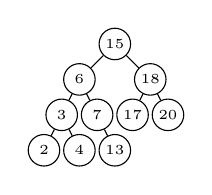
\begin{tikzpicture}[scale=0.45,
        level distance=1cm,
        level 1/.style={sibling distance=2cm},
        level 2/.style={sibling distance=1cm},
        every node/.style={circle,draw,inner sep=1pt,font=\tiny,minimum size=0.4cm}]
        
        % Example tree for predecessor
        \node {15}
            child {
                node {6}
                child {
                    node {3}
                    child {node {2}}
                    child {node {4}}
                }
                child {
                    node {7}
                    child[missing]
                    child {node {13}}
                }
            }
            child {
                node {18}
                child {node {17}}
                child {node {20}}
            };
    \end{tikzpicture}
    \caption*{\footnotesize Example: Predecessor of 15 is 13 (maximum in left subtree)}
\end{figure}

\textbf{Explanation:}
\begin{itemize}
    \item Case 1: If $x$ has a left subtree, the predecessor is the maximum element in that subtree
    \item Case 2: If no left subtree exists, we go up the tree until we find a node that is a right child
    \item The predecessor's key is the largest key in the tree smaller than $x.key$
\end{itemize}

\subsection{Exercise 3.4: Binary Search Tree Insertion}
\textbf{Problem:} Let $T$ be a Binary Search Tree. Prove that it always possible to insert a node $z$ as a leaf of the tree $T$ with $z.key = r$.

\textbf{Solution:} This is a straightforward property of Binary Search Trees. We prove this by induction on the height of the tree.

\begin{proof}
\begin{itemize}
\item \textbf{Base case} ($h = 0$):
    \begin{itemize}
        \item Tree consists only of root node $x$
        \item If $r \leq x.key$: place $z$ as left child of $x$
        \item If $r > x.key$: place $z$ as right child of $x$
    \end{itemize}

\item \textbf{Inductive step:}
    \begin{itemize}
        \item Assume the statement is true for trees of height $h-1$
        \item For a tree of height $h$ with root $x$:
        \begin{itemize}
            \item If $r \leq x.key$: insert in left subtree
            \item If $r > x.key$: insert in right subtree
        \end{itemize}
        \item By inductive hypothesis, we can insert in the chosen subtree (height $h-1$)
    \end{itemize}
\end{itemize}
\end{proof}

\begin{figure}[H]
    \centering
    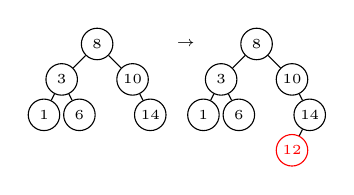
\begin{tikzpicture}[scale=0.45,
        level distance=1cm,
        level 1/.style={sibling distance=2cm},
        level 2/.style={sibling distance=1cm},
        every node/.style={circle,draw,inner sep=1pt,font=\tiny,minimum size=0.4cm}]
        
        % Before insertion
        \node {8}
            child {
                node {3}
                child {node {1}}
                child {node {6}}
            }
            child {
                node {10}
                child[missing]
                child {node {14}}
            };
            
        % Arrow
        \node[draw=none] at (2.5,0) {$\rightarrow$};
        
        % After insertion of 12
        \begin{scope}[xshift=4.5cm]
        \node {8}
            child {
                node {3}
                child {node {1}}
                child {node {6}}
            }
            child {
                node {10}
                child[missing]
                child {
                    node {14}
                    child {node[red] {12}}
                    child[missing]
                }
            };
        \end{scope}
    \end{tikzpicture}
    \caption*{\footnotesize Example: Inserting node with key=12 (shown in red)}
\end{figure}

\textbf{Key Points:}
\begin{itemize}
    \item The BST property ensures we can always find a valid leaf position
    \item At each step, we reduce the problem to a smaller subtree
    \item The process terminates when we reach a NULL child pointer
    \item Insertion maintains the BST property
\end{itemize}

\subsection{Exercise 3.5: Binary Search Tree Deletion}
\textbf{Problem:} Let $T$ be a Binary Search Tree given in the figure below. Give the output tree after the call of TREE-DELETE$(T, z)$ where $z$ is the node with key 41.

\begin{figure}[H]
    \centering
    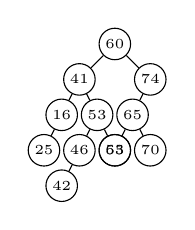
\begin{tikzpicture}[scale=0.45,
        level distance=1cm,
        level 1/.style={sibling distance=2cm},
        level 2/.style={sibling distance=1cm},
        every node/.style={circle,draw,inner sep=1pt,font=\tiny,minimum size=0.4cm}]
        
        % Initial tree
        \node {60}
            child {
                node {41}
                child {
                    node {16}
                    child {node {25}}
                    child[missing]
                }
                child {
                    node {53}
                    child {
                        node {46}
                        child {node {42}}
                        child[missing]
                    }
                    child {node {55}}
                }
            }
            child {
                node {74}
                child {
                    node {65}
                    child {node {63}}
                    child {node {70}}
                }
                child[missing]
            };
    \end{tikzpicture}
    \caption*{\footnotesize Initial Binary Search Tree with node 41 to be deleted}
\end{figure}

\textbf{Algorithm: TREE-DELETE$(T,z)$}
\begin{algorithm}[H]
\begin{algorithmic}[1]
\Procedure{Tree-Delete}{$T,z$}
    \If{$z.left = \text{NIL}$}
        \State \textsc{Transplant}$(T,z,z.right)$
    \ElsIf{$z.right = \text{NIL}$}
        \State \textsc{Transplant}$(T,z,z.left)$
    \Else
        \State $y \gets \text{Tree-Minimum}(z.right)$
        \If{$y.p \neq z$}
            \State \textsc{Transplant}$(T,y,y.right)$
            \State $y.right \gets z.right$
            \State $y.right.p \gets y$
        \EndIf
        \State \textsc{Transplant}$(T,z,y)$
        \State $y.left \gets z.left$
        \State $y.left.p \gets y$
    \EndIf
\EndProcedure
\end{algorithmic}
\end{algorithm}

\textbf{Solution:} Let's solve this step by step following the TREE-DELETE algorithm:

\begin{enumerate}
    \item \textbf{Analyze the node to be deleted (41):}
        \begin{itemize}
            \item Node 41 has two children: 16 (left) and 53 (right)
            \item Since it has two children, we fall into the third case (lines 7-15)
            \item We need to find its successor to replace it
        \end{itemize}
    
    \item \textbf{Find the successor of 41 (lines 7):}
        \begin{itemize}
            \item Call TREE-MINIMUM$(z.right)$ to find successor
            \item Right subtree starts at node 53
            \item Follow left pointers: 53 → 46 → 42
            \item Node 42 has no left child, so it's the successor
        \end{itemize}
    
    \item \textbf{Handle successor's position (lines 8-11):}
        \begin{itemize}
            \item Check if successor (42) is not a direct child of 41
            \item Since 42 is not direct child (it's grandchild), we:
                \begin{itemize}
                    \item Replace 42 with its right child (NIL in this case)
                    \item Make 42 point to 41's right child (53)
                    \item Make 53's parent point to 42
                \end{itemize}
        \end{itemize}

    \item \textbf{Complete the replacement (lines 12-14):}
        \begin{itemize}
            \item Replace 41 with 42 using TRANSPLANT
            \item Make 42 point to 41's left child (16)
            \item Make 16's parent point to 42
        \end{itemize}
\end{enumerate}

\begin{figure}[H]
    \centering
    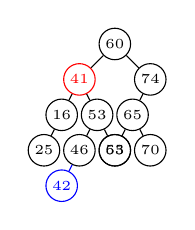
\begin{tikzpicture}[scale=0.45,
        level distance=1cm,
        level 1/.style={sibling distance=2cm},
        level 2/.style={sibling distance=1cm},
        every node/.style={circle,draw,inner sep=1pt,font=\tiny,minimum size=0.4cm}]
        
        % Intermediate step - finding successor
        \node {60}
            child {
                node[red] {41}
                child {
                    node {16}
                    child {node {25}}
                    child[missing]
                }
                child {
                    node {53}
                    child {
                        node {46}
                        child[blue] {node {42}}
                        child[missing]
                    }
                    child {node {55}}
                }
            }
            child {
                node {74}
                child {
                    node {65}
                    child {node {63}}
                    child {node {70}}
                }
                child[missing]
            };
    \end{tikzpicture}
    \caption*{\footnotesize Finding successor: Node to delete (41) in red, successor (42) in blue}
\end{figure}

\begin{figure}[H]
    \centering
    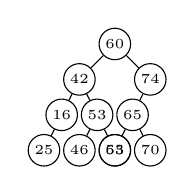
\begin{tikzpicture}[scale=0.45,
        level distance=1cm,
        level 1/.style={sibling distance=2cm},
        level 2/.style={sibling distance=1cm},
        every node/.style={circle,draw,inner sep=1pt,font=\tiny,minimum size=0.4cm}]
        
        % Final tree after deletion
        \node {60}
            child {
                node {42}
                child {
                    node {16}
                    child {node {25}}
                    child[missing]
                }
                child {
                    node {53}
                    child {
                        node {46}
                    }
                    child {node {55}}
                }
            }
            child {
                node {74}
                child {
                    node {65}
                    child {node {63}}
                    child {node {70}}
                }
                child[missing]
            };
    \end{tikzpicture}
    \caption*{\footnotesize Final Binary Search Tree after deleting node 41}
\end{figure}

\textbf{Key Points for Tree Deletion:}
\begin{itemize}
    \item There are three cases when deleting a node:
        \begin{enumerate}
            \item Node has no children (leaf node):
                \begin{itemize}
                    \item Simply remove it by setting parent's pointer to NIL
                    \item Example: Deleting a leaf like node 25
                \end{itemize}
            
            \item Node has one child:
                \begin{itemize}
                    \item Replace node with its only child
                    \item Update parent pointers
                    \item Example: If node 16 had only child 25
                \end{itemize}
            
            \item Node has two children:
                \begin{itemize}
                    \item Find successor (smallest value in right subtree)
                    \item Replace node with successor
                    \item Handle successor's original position
                    \item Example: Node 41 in our case
                \end{itemize}
        \end{enumerate}
    
    \item Finding the successor (TREE-MINIMUM):
        \begin{itemize}
            \item Start at node's right child
            \item Keep following left pointers until NIL
            \item Last node found is successor
            \item Important: Successor never has a left child
        \end{itemize}
    
    \item TRANSPLANT operation:
        \begin{itemize}
            \item Used to replace one subtree with another
            \item Updates parent pointers correctly
            \item Handles special case of root node
            \item Does not handle child pointers of moved nodes
        \end{itemize}
\end{itemize}

\textbf{Verification:} After deletion:
\begin{itemize}
    \item Node 42 maintains BST property:
        \begin{itemize}
            \item Left subtree (16, 25) contains values < 42
            \item Right subtree (53, 46, 55) contains values > 42
        \end{itemize}
    \item Tree structure remains valid:
        \begin{itemize}
            \item All parent-child pointers are correct
            \item No nodes were lost or duplicated
        \end{itemize}
    \item BST invariants are preserved:
        \begin{itemize}
            \item For every node: left subtree values < node key < right subtree values
            \item Tree remains connected
            \item No cycles are created
        \end{itemize}
\end{itemize}
